\section{Vstupní zařízení}
\label{sec:vstupni-zarizeni}
\subsection{Klávesnice}
Klávesenice předává informace o stlačených klávesách operačnímu systému zpracované BIOSem.
Připojují se fyzicky pomocí USB a PS2 konektoru nebo bezdrátově pomocí Bluetooth či infračerveného záření.
Informace jsou ve SCAN kódu, kde se začíná klávesou ESC na čísle 1 a pokračuje se dál po řádcích.
Postup přenosu stisku:\\
\begin{enumerate}
  \item Mikroprocesor vestavěný do klávesnice nebo základové desky neustále monitoruje stav klávesnice
  \item Změna stavu způsobí vysílání kódu do základové desky klávesnice
  \item Stisk musí trvat aspoň 2 nebo 3 cykly, jinak se ignoruje
  \item Po uvolnění klávesy se kód klávesy zvýší o 128
  \item Číslo se uloží do paměti klávesnice a mikroprocesorem se zapíše na port
  \item Nastane přerušení a BIOS čte kód klávesy
  \item Po přečtení BIOS sdělí klávesnici pokyn o vymazání klávesy
  \item Při delším stisku se generuje signál stlačené klávesy
  \item BIOS dále testuje ještě 2 byty klávesnice na portu pro případné speciální funkce jako CTRL, ALT, aj.\\
        Tyto funkce se zapisují do bytů na adrese 0417H a 0418H
\end{enumerate}
\subsubsection{Mechanické klávesnice}
Potlačením tlačítka se mechanicky spojí vodiče. Pružinou se klávesa vratí zpátky.\\
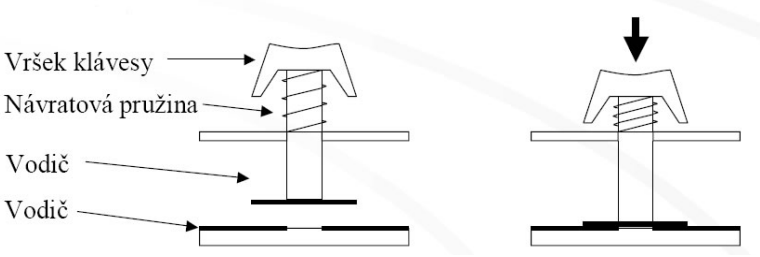
\includegraphics[width=1\linewidth]{TVY-POS/Vstupni-zarizeni/mechanickey.png}
\subsubsection{Membránové klávesnice}
Protlačením membrány dojde ke styku kontaků. Většinou pomocí mikrospínačů.\\
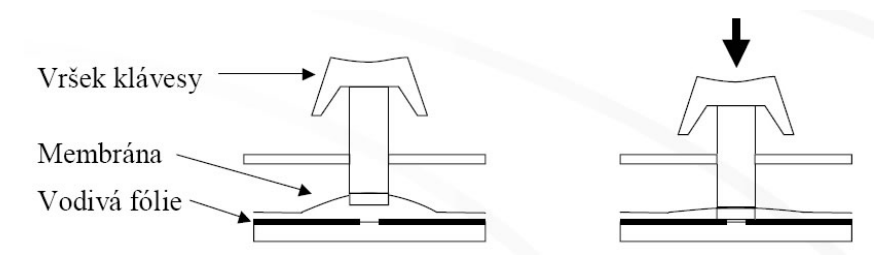
\includegraphics[width=1\linewidth]{TVY-POS/Vstupni-zarizeni/membranekey.png}
\subsubsection{Kapacitní klávesnice}
Přiblížení jádra k dorazu změní kapacitu kondnzátoru.
Není zde žádný dotek.
Jádrem je dielektrikum, které je pružinou oddalování.\\
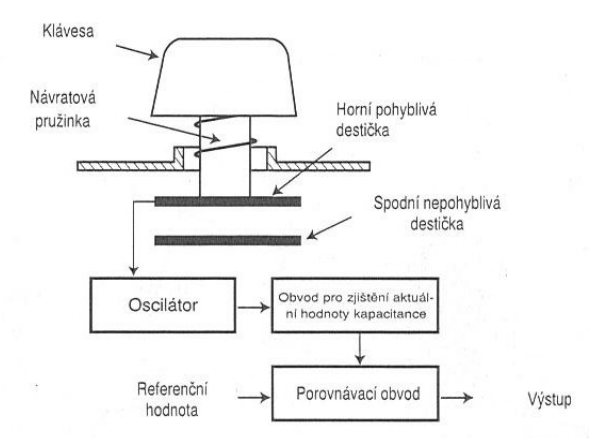
\includegraphics[width=1\linewidth]{TVY-POS/Vstupni-zarizeni/capacitorkey.png}
\subsubsection{Hallovy klávevy}
Klávesy mají uvnitř permanentní magnet.
Pod klávesou je Hallova sonda, která reguje za změnu magentického pole.
Při stisku klávesy se magnet přiblíží k Hallově sondě, která jako reakci vyšle elektrický signál.
Změnou magnetického pole pohybem klávesy se změní napětí na výstupu.
Takové klávesnice jsou velmi kvalitní, ale drahé.
\subsubsection{Dotykové klávesnice}
Dotyky se detekují pomocí změny kapacity kondenzátoru změnou dielektrika, který představuje prst.
Bez pohyblivých částí.
\subsection{Tablety}
Jsou to snímací podložky funkčně podobné grafickým stolům.
Využívají se ke kreslení vektorových obrazců.
Po podložce se pohybuje snímací zařízení, většinou myš se zaměřovačem nebo pero.
Myš místo kuličky obsahuje vysílací cívku, která vysílá impulsy čtené podložkou pomocí sítě snímačů.
Obsahuje lupu pro přenou polohu a tlačítka.
V peru bývá tlakový senzor pro určení tloušťky čáry.
\subsection{Světelná pera (Optická, Light Pen)}
Světelné pero snímá pozici pera na monitoru pomocí grafického adaptéru.
V peru je snímač světla, který identifikuje polohu pomocí bodu na monitoru.
Pracuje s informací, kdy se bod na monitoru obnoví, pomocí které určí, kde se pero nachází.
Monitor musí obraz vysílat řádek po řádku, bod po bodu.
\subsection{Dotykové obrazovky}
Existuje několik druhů dotykových obrazovek
\subsubsection{Rezistivní displeje}
Obrazovku tvoří pružná membrána.
Stiskem membrány spojíme elektrický proud.
Na základě velikosti jednotlivých proudů se vypočítá poloha displeje.
\subsubsection{Kapacitní dotykové dispeje}
Funguje na základě vodivosti lidského těla.
Dotykem prstu na displej se uzavře elektrický obvod a vytvoří se kapacita.
Řadič na základě velikosti kapacity určí polohu prstu.
\subsubsection{Dotykové displeje s IR}
Kolem displeje je rám vysílající IR paprsky.
Vsunutím předmětu se paprsek na daném místě přeruší.
\subsubsection{Displej s povrchovou akustickou vlnou (SAW)}
V rozích displeje jsou vysílače a přjímače 5Mhz sígnálu.
Přijímače vyhodnucují změnu šíření těchto vln a podle toho vyhodnutí polohu rušení.
Problematická je citlivost, jelikož malé znečištění je stále fatální.
\subsection{Myši}
Je to malé polohovací zařízení, která přenáší informace o svém pohybu do počítače.
Většinou se toto projeví jako pohyb kruzoru.
Mívá tlačíka a kolečko.
Připojovala se pomocí sériového RS-232 portu, poté se používal PS/2 a nyní USB.
Některé myši se dají pomocí redukce připojit do PS/2 či USB.
Existují i bezdrátové myši, u kterých se využívá buďto IR (IrDA) nebo rádiových vln (Např.: Bluetooth).
\subsubsection{Mechanická myš (Kuličková)}
Zespod myši je kulička, která se pohybem roztáčí.
Otáčení kuličky snímají dvě navzájem kolmé hřídele, na kterých se nachází dvě dvojice snímačů.
Hřídele při svém pohybu přenáší pohyb na otočnou clonu ve tvaru kruhu s okny.
Každé pootočení clony přeruší paprsek, což je přeneseno na elektrický impulz.
Rozpoznává se směr otáčení pomocí Grayova kódu.
Impulzy myši tvoří 2 a 2 bity, která se pak převádí na pohyb po X a Y na obrazovce.
\subsubsection{Optická myš}
Myš vysílá LED nebo laser, který se snímá fotodiodami nebo jiným optickým snímačem.
Pohyb myši se poté v reálném čase převádí do os X a Y.
Infračervené záření má vyšší přesnost a nižší spotřebu, ale ve skutečnosti na světle nezáleží.
Myš funguje lépe na strukturovaném povrchu, kde je možné snadno rozpoznat pohyb podkladu.
